\section{Admissible invariant distributions: local regularity, descent, and spectral finiteness}\label{sec:descent}
The preceding sections distinguish algebraic spectral data from their topological completions. We now ask what such data imply locally on the group. The important point is that the size of the Laurent moments at infinity need not govern singular behavior on compact subsets. We continue to assume that $F$ is a $p$-adic field of odd residual characteristic.

\subsection{Admissibility and local regularity}
For compact open subgroups $K'\subset K$ and an irreducible smooth representation $\sigma$ of $K'$, let
\[
e_\sigma(k)=\frac{\dim\sigma}{\operatorname{vol}(K')}
 \operatorname{tr}\sigma(k^{-1})\quad(k\in K'),
\]
extended by zero. With Haar measure on $G$ this is the central isotypic idempotent in the convolution algebra of $K'$. Say that $\sigma$ intertwines the trivial type on $K$ in $G$ if for some $g\in G$ its restriction to $K'\cap gKg^{-1}$ contains the trivial representation.

We use the local admissibility condition of the original notes: an invariant distribution $D$ is $(G,K)$-admissible at $\gamma$ if $D(f*e_\sigma)=0$ for all $f$ supported in $\gamma K$, all $K'\subset K$, and all $\sigma$ not intertwining the trivial type on $K$. In this formulation one may use the contragredient idempotent instead, with the corresponding change of type label. The intertwining condition with the trivial type is unchanged. Admissibility on an invariant open set means that such a $K$ exists at every point of the set.

The Harish-Chandra regularity input used below is that irreducible admissible characters satisfy the local condition, and admissible invariant distributions have locally integrable invariant representatives, locally constant on the regular semisimple set and with locally bounded discriminant-normalized density. See \cite{HC99} for the regularity theory; the precise hypotheses and formulation in that source require a source-level audit (Remark 2026.8). We use the condition at every point, not only at regular points.

\begin{lemma}\label{lem:admissibility-local}
The local admissibility condition is preserved by shrinking $K$, taking finite linear combinations of admissible distributions, and replacing a distribution by one agreeing with it on all test functions in an open neighborhood of $\gamma$.
\end{lemma}
\begin{proof}
If a type of a smaller subgroup intertwines the trivial representation on $K$, the same intertwining element works after $K$ is shrunk: the intersection on which invariance is required decreases. Thus failure to intertwine the smaller trivial type implies failure to intertwine the larger one. Also $\gamma K_1\subset\gamma K$ when $K_1\subset K$. This proves the first assertion. For finitely many distributions take a common smaller subgroup and use linearity. Finally choose $K$ with $\gamma K$ contained in the neighborhood of agreement. For $K'\subset K$, convolution on the right by $e_\sigma$ preserves the support condition in $\gamma K$. The defining test therefore takes the same value on both distributions.
\end{proof}

Representability by a locally integrable function, local constancy on the regular set, and a locally bounded normalized density are distinct from global temperedness. In particular, a point mass at the identity is invariant but is not represented by a locally integrable function. We will return to this example below.

\subsection{Local finite-character interpolation}
Let $\mathfrak s$ be a principal-series Bernstein component. Fix the restriction $\xi$ of an inducing character to $\mathcal O^\times$ and use $\chi_{\xi,z}(\varpi^m a)=z^m\xi(a)$. For a regular split element $a(t)$ with $t=\varpi^m a$, the total induced character is
\[
\Theta_{I(\chi_{\xi,z})}(a(t))=
\frac{\xi(a)z^m+\xi(a)^{-1}z^{-m}}{|t-t^{-1}|}.
\]
It is zero on the regular elliptic set. This is a formula for the full induced character even at reducible parameters.

\begin{lemma}\label{lem:compact-exponents}
For every compact subset $C$ of $G$, the integers $v(t)$ occurring among split eigenvalues of regular elements of $C$ form a bounded set.
\end{lemma}
\begin{proof}
The traces of matrices in $C$ are bounded in absolute value. If $|t|\ne1$, the ultrametric inequality gives $|t+t^{-1}|=\max(|t|,|t|^{-1})=q^{|v(t)|}$. If $|t|=1$, the valuation is zero. This gives a common bound.
\end{proof}

\begin{theorem}[Local finite-character interpolation]\label{thm:local-interpolation}
Assume the classical character formula and local integrability of irreducible characters. Let $L$ be an arbitrary algebraic linear functional on the Laurent-polynomial total-trace coordinate of a principal-series block (with Weyl invariance where appropriate). Define $D_L(f)=L(z\mapsto\operatorname{tr}I(\chi_{\xi,z})(f))$. On every relatively compact open set $V$ in $G$, this distribution is a finite linear combination of irreducible tempered character distributions. The combination may depend on $V$. Its regular invariant density is zero on the elliptic set, and on the split set equals
\[
F_L(a(t))=
\frac{\xi(a)L(z^m)+\xi(a)^{-1}L(z^{-m})}{|t-t^{-1}|}
\]
in a non-Weyl-invariant block. In a Weyl-invariant block the numerator is evaluated as a single invariant Laurent polynomial.
\end{theorem}
\begin{proof}
Put $C=\overline V$. By Lemma~\ref{lem:compact-exponents}, the numerators on $C$ lie in the finite-dimensional space of Laurent polynomials with exponents between $-M$ and $M$ for some $M$. In the self-inverse case intersect this space with the Weyl-invariant subspace. Call the resulting space $P_M$.

Evaluation at generic points of the unit circle spans $P_M^*$: otherwise a nonzero Laurent polynomial would vanish at every such point, contradicting the polynomial identity theorem. Choose a finite spanning set of evaluations at parameters $z_j$, avoiding the finitely many reducibility points, and constants $c_j$ with $L|_{P_M}=\sum_j c_j\operatorname{ev}_{z_j}$.

For $f$ supported in $V$, the induced trace polynomial belongs to $P_M$. To see this without assuming interchange with an infinite functional, first multiply the pointwise numerator by $f$ and integrate the finitely many coefficient functions. These coefficient functions are locally integrable on $C$: they are fixed linear combinations of the finitely many generic induced character functions, obtained from an injective evaluation matrix on $P_M$. The regular semisimple complement is Haar-null, so the character integral for each $z$ equals the integral of this finite expansion. This proves the asserted polynomial membership and the identity
\[
D_L(f)=\sum_j c_j\Theta_{I(\chi_{\xi,z_j})}(f).
\]
The parameters are unitary and irreducible, hence tempered. The same finite interpolation gives the displayed pointwise formula on the regular set in $V$. Exhaustion by relatively compact open sets gives a locally integrable representative on $G$; the representatives agree on overlaps up to null sets, and their regular formulas agree pointwise.
\end{proof}

For $\xi=1$, put $m_n=L(B_n)$, with $B_0=1$. The formula simplifies to
\[
F_L(a(t))=\frac{1}{|t-t^{-1}|}
\begin{cases}
m_{|v(t)|},&v(t)\ne0,\\
2m_0,&v(t)=0.
\end{cases}
\]
The constant mode is indispensable. On compact sets the normalized density is bounded, since only finitely many moments occur there.

\begin{theorem}[Finite Bernstein support]\label{thm:finite-block-admissibility}
Assume the algebraic block descriptions in Section~\ref{sec:pwcomparison} and the Harish-Chandra character admissibility input above. Every invariant distribution with finite Bernstein spectral support satisfies the local admissibility condition and is locally representable. No global bound on its Laurent moments is needed.
\end{theorem}
\begin{proof}
In a principal-series block, decompose its spectral functional into the continuous-family functional $L$ and the two exceptional coefficients when present. The latter are finite combinations of irreducible characters. Each supercuspidal block is a single character coordinate since $G$ has no nontrivial unramified characters. Theorem~\ref{thm:local-interpolation} represents the $L$ contribution locally as a finite sum of characters. There are finitely many blocks by hypothesis, so the total sum is finite on each relatively compact open set. Lemma~\ref{lem:admissibility-local} and character admissibility give the assertion. Local integrability and the normalized bound follow either from the finite character formula or from regularity.
\end{proof}
The theorem is conditional on the stated classical inputs, not a new assertion of a general regularity theorem. In particular it does not follow from finite Bernstein support of a multiplier merely by treating that multiplier as a finite spectral sum.

\begin{center}
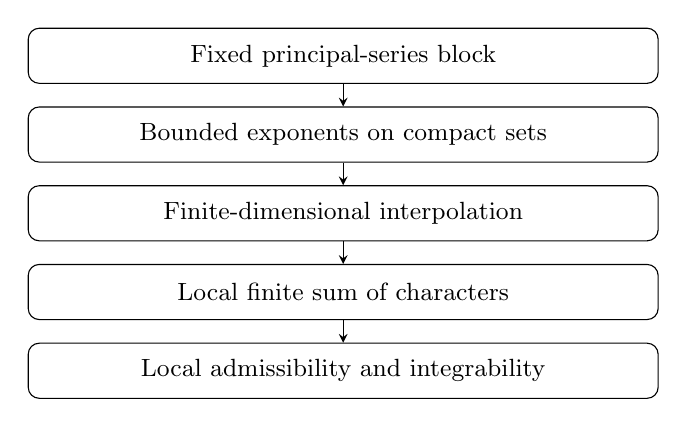
\begin{tikzpicture}[>=stealth,every node/.style={font=\small}]
\foreach \y/\t in {4/{Fixed principal-series block},3/{Bounded exponents on compact sets},2/{Finite-dimensional interpolation},1/{Local finite sum of characters},0/{Local admissibility and integrability}}{
\node[draw,rounded corners,minimum width=8cm,minimum height=7mm] (v\y) at (0,\y) {\t};}
\foreach \a/\b in {4/3,3/2,2/1,1/0}{\draw[->] (v\a)--(v\b);}
\end{tikzpicture}
\end{center}

\begin{example}
In the unramified block take $m_n=n!$ for $n\ge1$ and any $m_0$, with the exceptional coefficients zero. The theorem proves local admissibility, whereas the Laurent criterion rules out extension to the punctured-plane holomorphic spectral space and to the smooth circle spectral space. The example separates local regularity from global analytic and tempered growth. The same construction works with $m_n=\exp(n^2)$, while $m_n=\exp(\sqrt n)$ extends to every open annular spectral space but not the smooth circle. The group-side temperedness conclusions use the smooth trace identification in the preceding sections.
\end{example}

\subsection{Three kinds of descent}
For a locally integrable invariant density $F_D$ that is locally constant on the regular set, distinguish its ordinary restriction to a torus, its normalized split restriction
\[
h_D(a)=|\Delta_G(a)|^{1/2}F_D(a),
\]
and the normalized Jacquet-module or constant-term constructions. The first two are initially functions on the regular torus; the third is representation-theoretic and involves asymptotic character theory \cite{Ca93,Si79}. The Weyl integration formula expresses the split part of $D(f)$ as
\[
\frac12\int_A h_D(a)F_f^A(a)\,da
\]
with compatible measures and normalized orbital integral $F_f^A$. This identity does not establish that $h_D$ is locally constant at singular points or that it is a Jacquet-module character. A locally constant function on the abelian torus defines an admissible distribution for the local type condition: choose a unit subgroup on which the density is constant; convolution with a nontrivial character of any smaller subgroup vanishes. Conversely the local condition for a torus forces a locally constant density there, by the finite Fourier decomposition of locally constant test functions on the chosen compact open coset.

\begin{example}[Failure of a general descent theorem]\label{ex:descent}
For the trivial representation, the normalized split restriction is $|t-t^{-1}|$. For $t=1+x$ sufficiently close to one, $t-t^{-1}=x(2+x)/(1+x)$, so the value is $|x|$ since $p>2$. At $t=1+\varpi^n$ the values are $q^{-n}$. They are distinct in every neighborhood of one. No locally constant extension at $1$ exists; the argument at $-1$ is analogous. Multiplication by the Weyl factor $1/2$ does not change this obstruction.
\end{example}
\begin{center}
\begin{tikzpicture}[x=.9cm,y=8cm,>=stealth]
\draw[->] (0,0)--(7.8,0) node[right]{$n$};
\draw[->] (0,0)--(0,.39) node[above]{$|t-t^{-1}|$};
\foreach \n in {1,...,7}{
\draw[teal,thick] (\n,0)--(\n,{3^(-\n)});
\fill[teal] (\n,{3^(-\n)}) circle (1.5pt);
\node[below] at (\n,0) {\n};}
\node[anchor=west] at (2,.27) {$t=1+3^n$ in $\mathbb Q_3$};
\end{tikzpicture}
\end{center}
On $A_{\rm reg}$ every normalized restriction of a locally constant regular density is locally constant: the nonzero discriminant has locally constant absolute value. The singular extension is the substantive issue.

\begin{theorem}[Descent for induced spectral functionals]\label{thm:induced-descent}
For an arbitrary algebraic functional on the total induced trace coordinate of a principal-series block, the normalized split density extends to a locally constant function on all of $A$.
\end{theorem}
\begin{proof}
By Theorem~\ref{thm:local-interpolation}, the normalized restriction is evaluation of $\xi(a)z^m+\xi(a)^{-1}z^{-m}$ by $L$. The valuation $m$ and the unit character $\xi(a)$ are locally constant, including in neighborhoods of $t=\pm1$. Thus the same expression defines the required extension at the singular points. In a Weyl-invariant block use the invariant numerator. For the unramified block the extension is constant on $\mathcal O^\times$, with value $2m_0$.
\end{proof}

\subsection{Exceptional constituents and the exact obstruction in the unramified block}
The following elementary restriction argument provides the needed split character identity. For a nontrivial quadratic character $\eta$, the normalized principal series of $\mathrm{GL}_2(F)$ induced from $(\eta,1)$ is irreducible by the classical $\mathrm{GL}_2$ reducibility criterion. Its restriction to $\mathrm{SL}_2(F)$ is $I(\eta)$: in the compact induced model this follows from $\mathrm{GL}_2(F)=\widetilde B\,\mathrm{SL}_2(F)$ and agreement of the normalized inducing characters on the Borel intersection. By the rank-one classification this restriction is the direct sum of two inequivalent irreducible representations $\pi_+,\pi_-$. Conjugation by $\mathrm{GL}_2(F)$ acts transitively on these two constituents, since a union of orbits of constituents would otherwise be a proper invariant subspace of the irreducible $\mathrm{GL}_2$ representation. The swapping element can be taken diagonal modulo $\mathrm{SL}_2(F)$, by using its determinant. Diagonal conjugation fixes $a(t)$. Hence the two regular character functions agree on the split regular set (conjugation preserves Haar measure on $\mathrm{SL}_2$, as is also seen from its adjoint determinant). In particular the quadratic difference has zero split normalized restriction. This argument uses the classical $\mathrm{GL}_2$ irreducibility and $\mathrm{SL}_2$ decomposition inputs, for which exact source verification remains necessary.

For Steinberg, trace additivity in $[I(|\cdot|)]=[\mathbf1]+[\mathrm{St}]$ yields
\[
h_{\mathrm{St}}(a(t))=|t|+|t|^{-1}-|t-t^{-1}|.
\]
Near either singular point this is $2-|t-t^{-1}|$.

\begin{theorem}[Unramified split descent criterion]\label{thm:unramified-descent}
Subject to the classical inputs just stated, a spectral functional $(L,\alpha,\beta)$ in the unramified block has a locally constant normalized split restriction on the full diagonal torus if and only if $\beta=0$, where $\beta$ is its coefficient of the independent Steinberg trace.
\end{theorem}
\begin{proof}
The $L$ contribution extends by Theorem~\ref{thm:induced-descent}. The quadratic difference contributes zero. Near one, the remaining contribution is $\beta(2-q^{-n})$ along $t=1+\varpi^n$. The $L$ contribution is constant along this sequence. If $\beta\ne0$ the resulting values cannot be eventually constant. Conversely, if $\beta=0$ both remaining contributions have locally constant extensions.
\end{proof}
For a ramified quadratic block, both exceptional differences have zero split restriction by the same swapping argument. Thus all principal-series block functionals in that block have locally constant normalized split descent. The theorem concerns a single block. For sums involving supercuspidal blocks the criterion is given in Corollary~\ref{cor:descent}, and the Steinberg obstruction can then cancel (Example~\ref{ex:cancel}).

\begin{center}
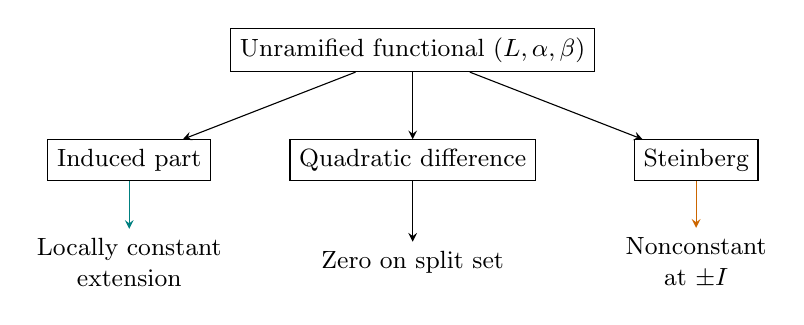
\begin{tikzpicture}[>=stealth,every node/.style={font=\small}]
\node[draw] (r) at (0,2.4) {Unramified functional $(L,\alpha,\beta)$};
\node[draw] (l) at (-3.6,1) {Induced part};
\node[draw] (d) at (0,1) {Quadratic difference};
\node[draw] (s) at (3.6,1) {Steinberg};
\foreach \v in {l,d,s}{\draw[->] (r)--(\v);}
\node[align=center] (lc) at (-3.6,-.3) {Locally constant\\extension};
\node (dc) at (0,-.3) {Zero on split set};
\node[align=center] (sc) at (3.6,-.3) {Nonconstant\\at $\pm I$};
\draw[->,teal] (l)--(lc);\draw[->] (d)--(dc);\draw[->,orange!80!black] (s)--(sc);
\end{tikzpicture}
\end{center}

\subsection{Character measures and higher spectral derivatives}
The original question about integrating characters is resolved for fixed finite Bernstein support by Theorem~\ref{thm:finite-block-admissibility}, rather than by assuming a uniform admissibility subgroup for an arbitrary family. A finite complex Borel measure on a compact tempered spectral subset of a block defines a functional by integration: for fixed $f$ the trace is bounded and Borel on the circle and at its finite exceptional points, by its polynomial coordinate and constituent values. Thus the integral exists. Finite support in the set of blocks makes the preceding theorem applicable. In the smooth block model the functional is continuous by the uniform norm estimate on the continuous coordinate and the ordinary finite-dimensional norms. This includes measures charging individual exceptional points, regardless of their Plancherel measure.

More generally, a distribution on the inducing unitary circle defines a spectral functional by pairing with the smooth total trace. It has finite distributional order on that compact circle. Theorem~\ref{thm:duality-moments} bounds its moments polynomially, and Theorem~\ref{thm:local-interpolation} supplies its local density. As an example take the $k$th angular derivative at $\theta_0$ of the total induced character. The unramified normalized split formula for $v(t)=m$ is
\[
2m^k\cos(m\theta_0+k\pi/2)
\]
for $k>0$, and $2\cos(m\theta_0)$ for $k=0$. For $k>0$ it vanishes on the regular split unit set. Such higher-order examples do not require a measure interpretation.

\subsection{Finite type and quasi-finite type}
The original notes express spectral distributions as derivatives of continuous functions on parameter tori. This can be retained in a precise Fourier form. For a bilateral sequence $m_n$ with polynomial bound of degree $N$, choose an integer $k>N+2$. After removing the constant mode, divide the Fourier coefficients of the distribution by $(in)^k$ for $n\ne0$. The resulting sequence is absolutely summable and hence defines a continuous periodic function. Its $k$th distributional derivative, plus the removed constant mode, is the original distribution (with Fourier sign conventions fixed consistently). The same argument applies to Weyl-invariant data by symmetrizing the derivative representation, or by choosing even $k$. The exceptional coordinates are separate scalars, not densities with respect to Plancherel measure.

We distinguish finite spectral type (finitely many nonzero blocks, each with polynomial moment growth), uniform quasi-finite spectral type (possibly infinitely many blocks but a common polynomial exponent, allowing block-dependent constants), and componentwise finite spectral order (each block has some polynomial exponent). These are refinements of the terminology of the original notes. The definition using derivatives of continuous functions also requires retaining the constant mode, and a uniform derivative order is equivalent to a uniform polynomial growth bound up to a fixed increase in the exponent.

\begin{center}
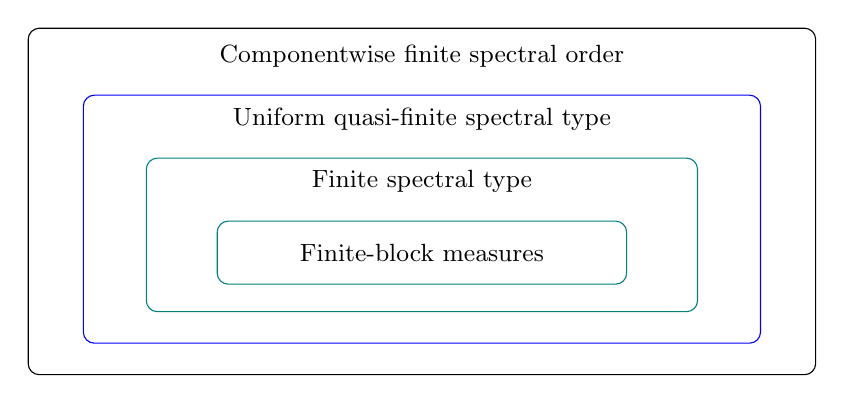
\begin{tikzpicture}[every node/.style={font=\small}]
\draw[rounded corners] (-5,-2.2) rectangle (5,2.2);
\node at (0,1.85) {Componentwise finite spectral order};
\draw[blue,rounded corners] (-4.3,-1.8) rectangle (4.3,1.35);
\node at (0,1.05) {Uniform quasi-finite spectral type};
\draw[teal,rounded corners] (-3.5,-1.4) rectangle (3.5,.55);
\node at (0,.25) {Finite spectral type};
\draw[teal,rounded corners] (-2.6,-1.05) rectangle (2.6,-.25);
\node at (0,-.65) {Finite-block measures};
\end{tikzpicture}
\end{center}
All three inclusions are strict at the spectral level. A derivative of a delta distribution on the circle need not be a finite measure, since its moments can be unbounded. Nonzero bounded sequences in infinitely many blocks give uniform quasi-finite but not finite type. Finally enumerate distinct generic ramified blocks by $\mathfrak s_j$, and take bilateral moments $m_{\mathfrak s_j,n}=n^{2j}$, $j\ge1$. Each block has finite order, but there is no uniform exponent. The interpretation of the last example as a group-side tempered distribution uses the global direct-sum topology and trace identification in Section~\ref{sec:tempered-duality}. The Plancherel measure need not be used as a reference measure for spectral distributions; multiplication or division by its density at singular points must be justified separately.

\subsection{Temperedness is not admissibility}
The point mass $\delta_I(f)=f(I)$ is invariant and continuous for the Schwartz topology: point evaluation is bounded by the defining seminorm on each fixed-level stage. It is not locally representable. Indeed, for a descending sequence of compact open neighborhoods $K_m$ of $I$, a locally integrable representative would satisfy $\int_{K_m}F(g)\,dg\to0$ by dominated convergence, while $\delta_I(\mathbf1_{K_m})=1$. Harish-Chandra regularity therefore rules out admissibility. By Plancherel inversion (with compatible Haar and Plancherel measures), it has the spectral expression
\[
\delta_I(f)=\int_{\widehat G_{\rm temp}}\Theta_\pi(f)\,d\mu_{\rm Pl}(\pi).
\]
The integral is the Plancherel trace formula, not a finite measure on the whole dual. Thus order zero on individual blocks does not guarantee local admissibility globally.

Conversely the trivial character is admissible but not tempered. The unramified polynomial moments of this character are $q^n+q^{-n}$ for $n\ge1$, with an independent coefficient $-1$ on the Steinberg trace. This violates the polynomial moment bound. This conclusion also follows directly from the ordinary non-temperedness of the trivial representation and the Schwartz trace theory.

\subsection{Central finiteness, block support and counterexamples}
Use the full Bernstein center, the product of the coordinate algebras of the components, acting on the algebraic trace space and its dual. Center-finite means that the orbit span of a functional under this center is finite-dimensional. The central block idempotents project a functional to its individual block components. Nonzero projections onto distinct blocks are linearly independent, so center-finiteness implies finite Bernstein support. By Theorem~\ref{thm:finite-block-admissibility}, it implies admissibility under the classical inputs of that theorem.

The converse fails. In the unramified block take
\[
L(Q)=\frac1{2\pi}\int_0^{2\pi}Q(2\cos\theta)\,d\theta,\qquad \alpha=\beta=0.
\]
This functional is a measure, is tempered in the smooth spectral model and is admissible by the finite-block theorem. If a nonzero polynomial $p$ annihilated $L$, taking $Q$ to have the conjugate coefficients of $p$ would give $\int |p(2\cos\theta)|^2\,d\theta=0$, a contradiction. Hence it is not center-finite. Center-finiteness does not imply temperedness either, as the trivial character illustrates.

\begin{center}
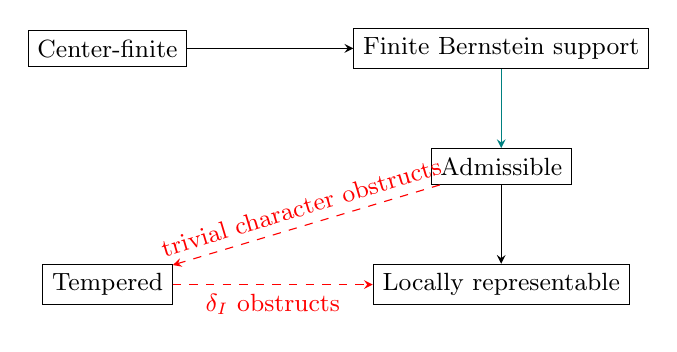
\begin{tikzpicture}[>=stealth,every node/.style={font=\small}]
\node[draw] (c) at (-3,2) {Center-finite};
\node[draw] (f) at (2,2) {Finite Bernstein support};
\node[draw] (a) at (2,.5) {Admissible};
\node[draw] (r) at (2,-1) {Locally representable};
\node[draw] (t) at (-3,-1) {Tempered};
\draw[->] (c)--(f);\draw[->,teal] (f)--(a);\draw[->] (a)--(r);
\draw[dashed,red,->] (t)--node[below] {$\delta_I$ obstructs}(r);
\draw[dashed,red,->] (a)--node[above,sloped] {trivial character obstructs}(t);
\end{tikzpicture}
\end{center}
Solid arrows denote implications using the indicated classical inputs; dashed red arrows denote false implications. Hecke-finiteness must be specified separately (for example by the precise fixed-level annihilation condition in a cited theorem). It is not a synonym for finite support or the proposed uniform quasi-finite spectral order. Its relation to center-finiteness in each block is discussed in Proposition~\ref{prop:hecke}.

\subsection{The original $\mathrm{GL}_2$ question}
The noncompact center in $\mathrm{GL}_2(F)$ motivates Fourier decomposition by central characters. For a test function $f$ and unitary central character $\omega$, the normalized central Fourier integral, when defined, is
\[
f_\omega(x)=\int_Z f(xz)\omega(z)^{-1}\,dz,\qquad
f_\omega(xz)=\omega(z)f_\omega(x).
\]
One cannot conclude that every distribution is an ordinary integral of pointwise distributions $D_\omega$; dependence on the central parameter may itself be distributional. Nor is a single global compact-open level automatic. A rank-two torus block suggests a corrected spectral model of smooth functions on $(S^1)^2$ with Weyl symmetry and the appropriate additional parameter spaces. Integration by parts and Fourier series give the elementary dual criterion
\[
|m_{j,k}|\le C(1+|j|+|k|)^N
\quad (j,k\in\mathbb Z).
\]
This is a torus calculation, not a proof of the full $\mathrm{GL}_2$ trace theorem. The original claim about quasi-finite representations of distributions is therefore retained as a research problem with invariant distributions and the actual topological trace space as necessary hypotheses.

\subsection{Remaining problems and literature}
The local interpolation theorem isolates the main rank-one input. Further work should check the exact Harish-Chandra admissibility definition and the classical character and restriction references, identify the full Schwartz topology, and investigate necessary conditions for admissibility of infinite-block distributions. In particular local finiteness of the character sums on open sets, not merely on individual test functions, is a useful candidate sufficient condition. Compare the normalized split restriction with normalized constant terms and Jacquet modules rather than identifying them at singular elements.

For broader context see Harish-Chandra \cite{HC99}, DeBacker's homogeneity results \cite{De02}, and the work on $\mathfrak z$-finite distributions by Aizenbud, Gourevitch and Sayag \cite{AGS15}. The recent preprint of Chen and Tsai \cite{CT26} on admissibility of Bernstein centers is particularly relevant to bounded spectral support. Its full text was not available for verification in the preceding literature pass; no theorem from it is used here. The relation between its center-valued distributions and the arbitrary scalar spectral functionals considered here must be checked. The group-side analytic growth question, the precise Hecke-finite formulation and the full $\mathrm{GL}_2$ extension remain open research directions rather than assertions of this paper.
